%****************************************************************************%
%* DIET User's Manual installing chapter file                               *%
%*                                                                          *%
%*  Author(s):                                                              *%
%*    - Eddy CARON (Eddy.Caron@ens-lyon.fr)                                 *%
%*    - Pushpinder Kaur Chouhan (Pushpinder.Kaur.Chouhan@ens-lyon.fr)       *%
%*    - Philippe COMBES (Philippe.Combes@ens-lyon.fr)                       *%
%*                                                                          *%
%* $LICENSE$                                                                *%
%****************************************************************************%
%* $Id$
%* $Log$
%* Revision 1.3  2005/06/24 09:15:11  rbolze
%* add missing file
%*
%* Revision 1.2  2005/06/23 22:53:36  rbolze
%* First version ...
%*
%* Revision 1.1  2005/06/14 08:04:59  ecaron
%* Dashboard section (Todo: Rapha�l)
%*
%* Revision 1.18  2005/05/29 13:51:22  ycaniou
%* Moved the section concerning FAST from description to a new chapter about FAST
%* and performances prediction.
%* Moved the section about convertors in the FAST chapter.
%* Modified the small introduction in chapter 1.
%* The rest of the changes are purely in the format of .tex files.
%*
%* Revision 1.17  2005/05/20 19:06:01  mjan
%* Short description of how to configure DIET for JuxMem
%*
%* Revision 1.16  2004/10/25 08:59:56  sdahan
%* add the multi-MA documentation
%*
%* Revision 1.15  2004/07/12 08:33:58  rbolze
%* explain how to copy cfgs file in install_dir/etc directory and correct my english
%*
%* Revision 1.14  2004/07/09 14:34:42  rbolze
%* make changes relative to DIET 1.1 version
%*
%* Revision 1.13  2004/07/06 13:40:42  ctedesch
%* add corrections from Raphael Bolze.
%*
%* Revision 1.12  2004/04/09 11:19:32  rbolze
%* Add the testing platform : Linux/amd64
%*
%* Revision 1.11  2004/04/05 11:04:29  rbolze
%* add instruction to compile with logService
%*
%* Revision 1.10  2004/02/10 00:13:55  ecaron
%* Add bugzilla reference.
%*
%* Revision 1.9  2004/01/29 17:08:47  ecaron
%* Add suggestions from Frederic Desprez. Thanks !
%*
%* Revision 1.8  2004/01/21 23:23:03  ecaron
%* Add suggestions from Jean-Yves. Thanks !
%*
%* Revision 1.7  2004/01/21 00:25:13  ecaron
%* Add suggestions from Holly Dail. Thanks !
%*
%* Revision 1.6  2004/01/07 20:25:04  ecaron
%* Add ScaLAPACK and BLAS introduction
%*
%* Revision 1.5  2004/01/06 15:07:46  ecaron
%* Correct latex bug
%*
%* Revision 1.4  2003/12/12 14:42:44  pkchouha
%*  define \diet_version in UserManual.tex to be 1.0
%*
%* Revision 1.3  2003/12/03 11:06:57  pkchouha
%* 1. change the version of DIET to 1.0
%* 2. DIET.tgz to DIET_1.0.tgz
%* 3. added the unlisted options in  section 2.2.1
%* 4. commented the  all part of section 2.2.2 before the subcetion oniORB
%* 5. added the unlisted options in section 2.2.2
%* 6. changed the args to conftest.c -o conftest
%* 7. changed some words and sentances for simplification
%*
%* Revision 1.2  2003/11/28 11:51:36  pcombes
%* Correction about gcc-2.96 management of exception handling.
%*
%* Revision 1.1  2003/09/09 12:38:20  pcombes
%* Reorganization of doc: UM becomes UsersManual.
%*
%* Revision 1.12  2003/06/23 13:14:09  pcombes
%* Update example to new configuration summary.
%*
%* Revision 1.11  2003/06/16 17:39:55  pcombes
%* One word about gcc-2.96.
%*
%* Revision 1.10  2003/06/02 13:47:05  pcombes
%* Fix footnotesize.
%*
%* Revision 1.9  2003/05/23 09:23:35  pcombes
%* Add suggestions from Jean-Yves. Thanks !
%*
%* Revision 1.8  2003/05/15 14:17:58  pcombes
%* UM 0.7
%*
%* Revision 1.6  2003/01/24 16:58:54  pcombes
%* UM 0.6.4
%*
%* Revision 1.5  2003/01/22 17:34:53  pcombes
%* User Manual, v. 0.6.4
%****************************************************************************%


\chapter{DIET dashboard}
\label{ch:dashboard}

\fixme{Rapha�l: Quelques mots sur DIET Dashboard + Screenshots}

%====[ Dependencies ]==========================================================
\section{LogService}
\label{sec:LogService}
%DIET use a third part software in order to be able to be monitored.
%We have choose to used LogService as monitoring system.
%LogService is a monitoring system which implement the three-thier model and offers
%a easy way to DIET components to be monitored.
%LogService use CORBA for all communication

The DIET platform can be monitored using a system called LogService %\cite{LogService}.
This monitoring service offers the capability to be aware of information that
you want to relay from the platform.
LogService (\ref{fig:DIET_LogService}) is composed of a set of three modules: \textit{LogComponent}, \textit{LogCentral} and \textit{LogTool}.
\begin{itemize}
 \item[-] \textit{LogComponent} attaches to a component and relays information and message
 to LogCentral
 \item[-] \textit{LogCentral} collects messages received from \textit{LogComponents},
 then \textit{LogCentral} stores or sends these messages to \textit{LogTools}.
 \item[-] \textit{LogTools} connect themselves to \textit{LogCentral} and wait for messages.
\end{itemize}
The main interest in LogService is that information is collected by
a central point \textit{LogCentral} that receives \textit{logEvents}
from \textit{LogComponents} that are attached to DIET elements ( MA, LA and SeD). The \textit{LogCentral}
offers the possibility to re-send this information to several tools (\textit{LogTools})
which are responsible for analysing these message and offering a comprehensive information
to the user.\\
\begin{figure}[htb]
  \begin{center}
    \resizebox{.6\linewidth}{!}{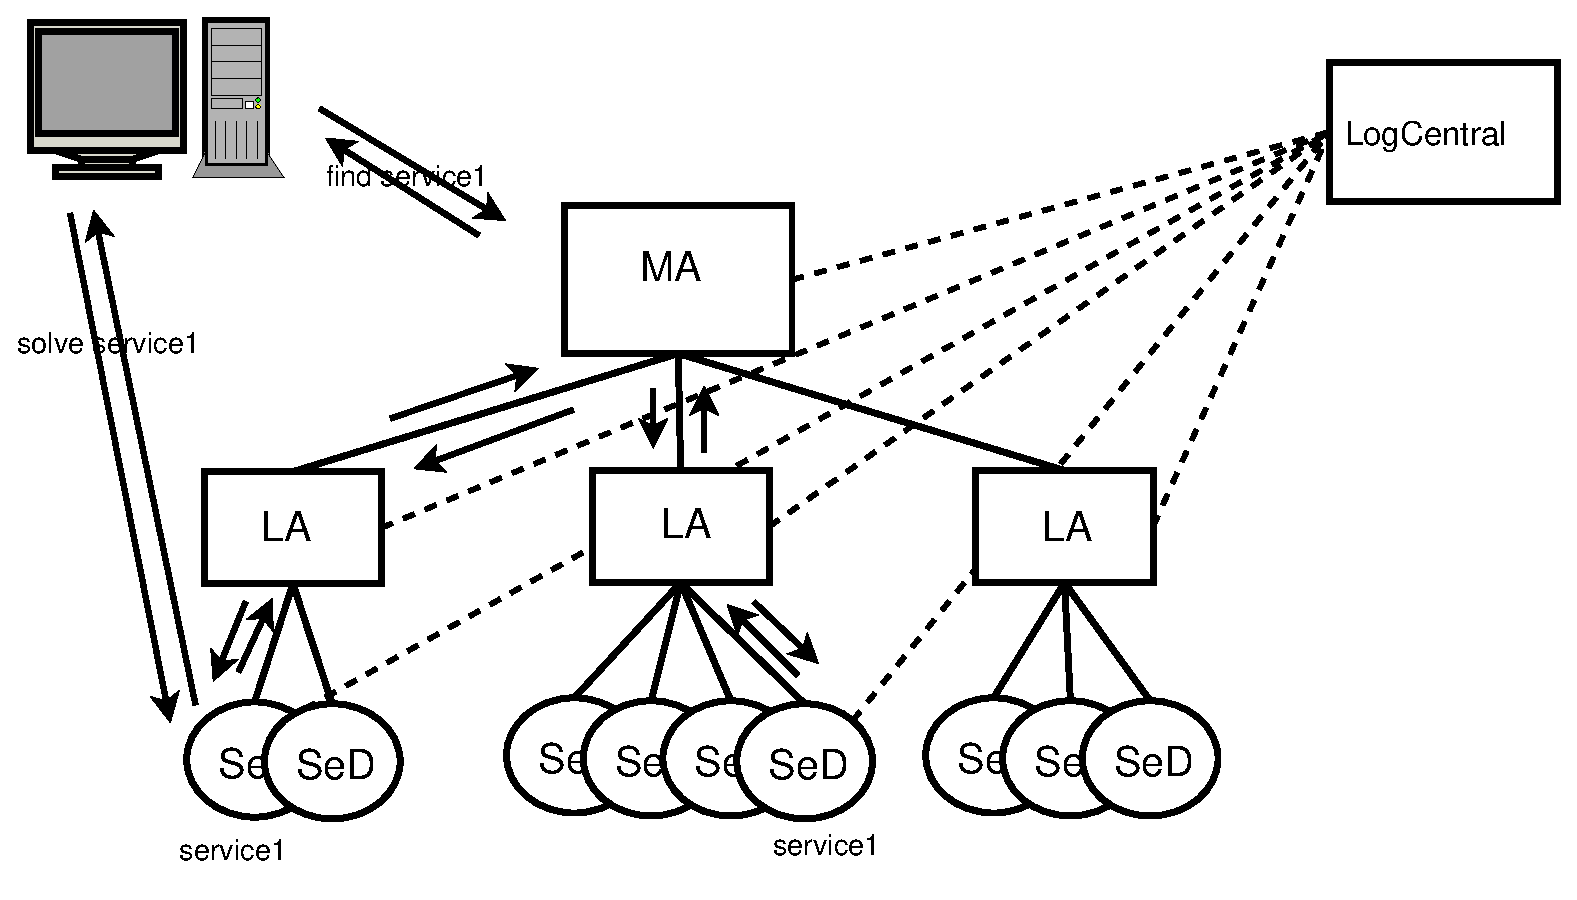
\includegraphics{fig/DIET_arch_request-2.ps}}
    \caption{DIET and LogService.}
    \label{fig:DIET_LogService}
  \end{center}
\end{figure}

LogService defines and implements several functionalities:
\begin{description}
  \item[Filtering mechanisms]
    As few messages as possible should be sent to
    minimize network traffic.  With respect to the three-tier model the communication,
    between applications and the monitor as well as tools and the monitor should be
    reduced to the minimum required.
    In order to decide which messages are required by a tool the tools have to
    declare their filter to the monitor (\textit{LogCentral}).
  \item[Message ordering]
    Event ordering is another important feature of a
    monitoring system. LogService handles this problem by the introduction of a global
    time line. At generation each message receives a time-stamp. The problem
    that can occur is that the system time can be different on each host.
    LogService measures this difference internally and corrects the time-stamps of
    incoming messages accordingly. The time difference is correcting by using the time stamp
    of the last ping that \textit{LogCentral} has send to \textit{LogComponent}.

    However, incoming messages are still unsorted. Thus, the messages are buffered
    for a short period of time in order to deliver a sorted stream of messages to
    the tools.  Messages that arrive out of order within this time are sorted in
    the buffer and can thus be properly delivered.  Although this induces a
    delivery-delay for messages, this mechanism guarantees the proper ordering 
    of messages within a certain tolerance.  As
    tools usually do not rely on true real-time delivery of messages this short
    delay is acceptable.
    
  \item[The System State Problem]
    A problem that arises in distributed environments is the state of the
    application. This state may for example contain information on connected
    servers, their relationships, the active tasks and many other pieces of
    information that depend on the application.  The system state can be
    constructed from all events that occurred in the application.  Some tools rely
    on this state to work properly.

    The problem emerges if those specific tools do not receive all messages.  This
    might occur as tools can connect to the monitor after the application has been
    started.  In fact, this is quite probable as the lifetime of the distributed
    application can be much longer than the lifetime of a tool.

    As a consequence, the system state must be maintained and stored.  In order to
    maintain a system state in a general way, LogService does not store the system
    state itself, but all messages which are required to construct it.  Those
    messages are identified by their tag and stored in a special list.  This list
    is forwarded to each tool that connects.  For the tool this process is
    transparent, since it simply receives a number of messages that represent the
    state of the application. \label{ref:LogService_system_stats}

    In order to further refine this concept, the list of important messages can
    also be cleaned up by LogService. This is necessary as components may connect
   and disconnect at runtime. After a disconnection of a component the respective
   information is no longer relevant for the system state.  Therefore, all
   messages which originated at this component can be removed from the list.  They
   have become obsolete due to the disconnection of the component and can be
   safely deleted in order to reduce the length of the list of important messages
   to a minimum.
\end{description}

All DIET components implement \textit{LogComponent} interface. By using LogCentral, the DIET
architecture is able to relay information to LogCentral, and then it is possible to connect to
LogCentral by using a \textit{LogTool} to collect, store and annalyse this information.



\section{VizDIET}
\label{sec:VizDIET}
VizDIET is the monitoring tool write for DIET to be able to vizualise and analyse the DIET 
architecture behaviors. As Describe in section \ref{sec:LogService}, all DIET's components 
integrete a \textit{LogComponent}, and VizDIET implement \textit{LogTool} interface in order to be 
able to collect all information send by DIET's components throught thier \textit{LogComponent}(see \ref{sec:LogService}).

VizDIET is able to draw a graphic representation of the DIET architecture monitored.
There are two way of using VizDIET.
\begin{description}
	\item[Real-time monitoring :] VizDIET is directly connected to the LogCentral, using
	a Corba connection. VizDIET recieved all messages from \textit{LogCentral} send by DIET
	component throught thier \textit{LogCompoent}.
	\item[Post-mortem monitoring :] VizDIET reads a log file where is stored all log
	messages recieved in \textit{LogCentral}. This post-mortem analysis can also be replayed
	in  real time if the log file is time sorted.
\end{description}

\begin{figure}[htb]
  \begin{center}
    \resizebox{.5\linewidth}{!}{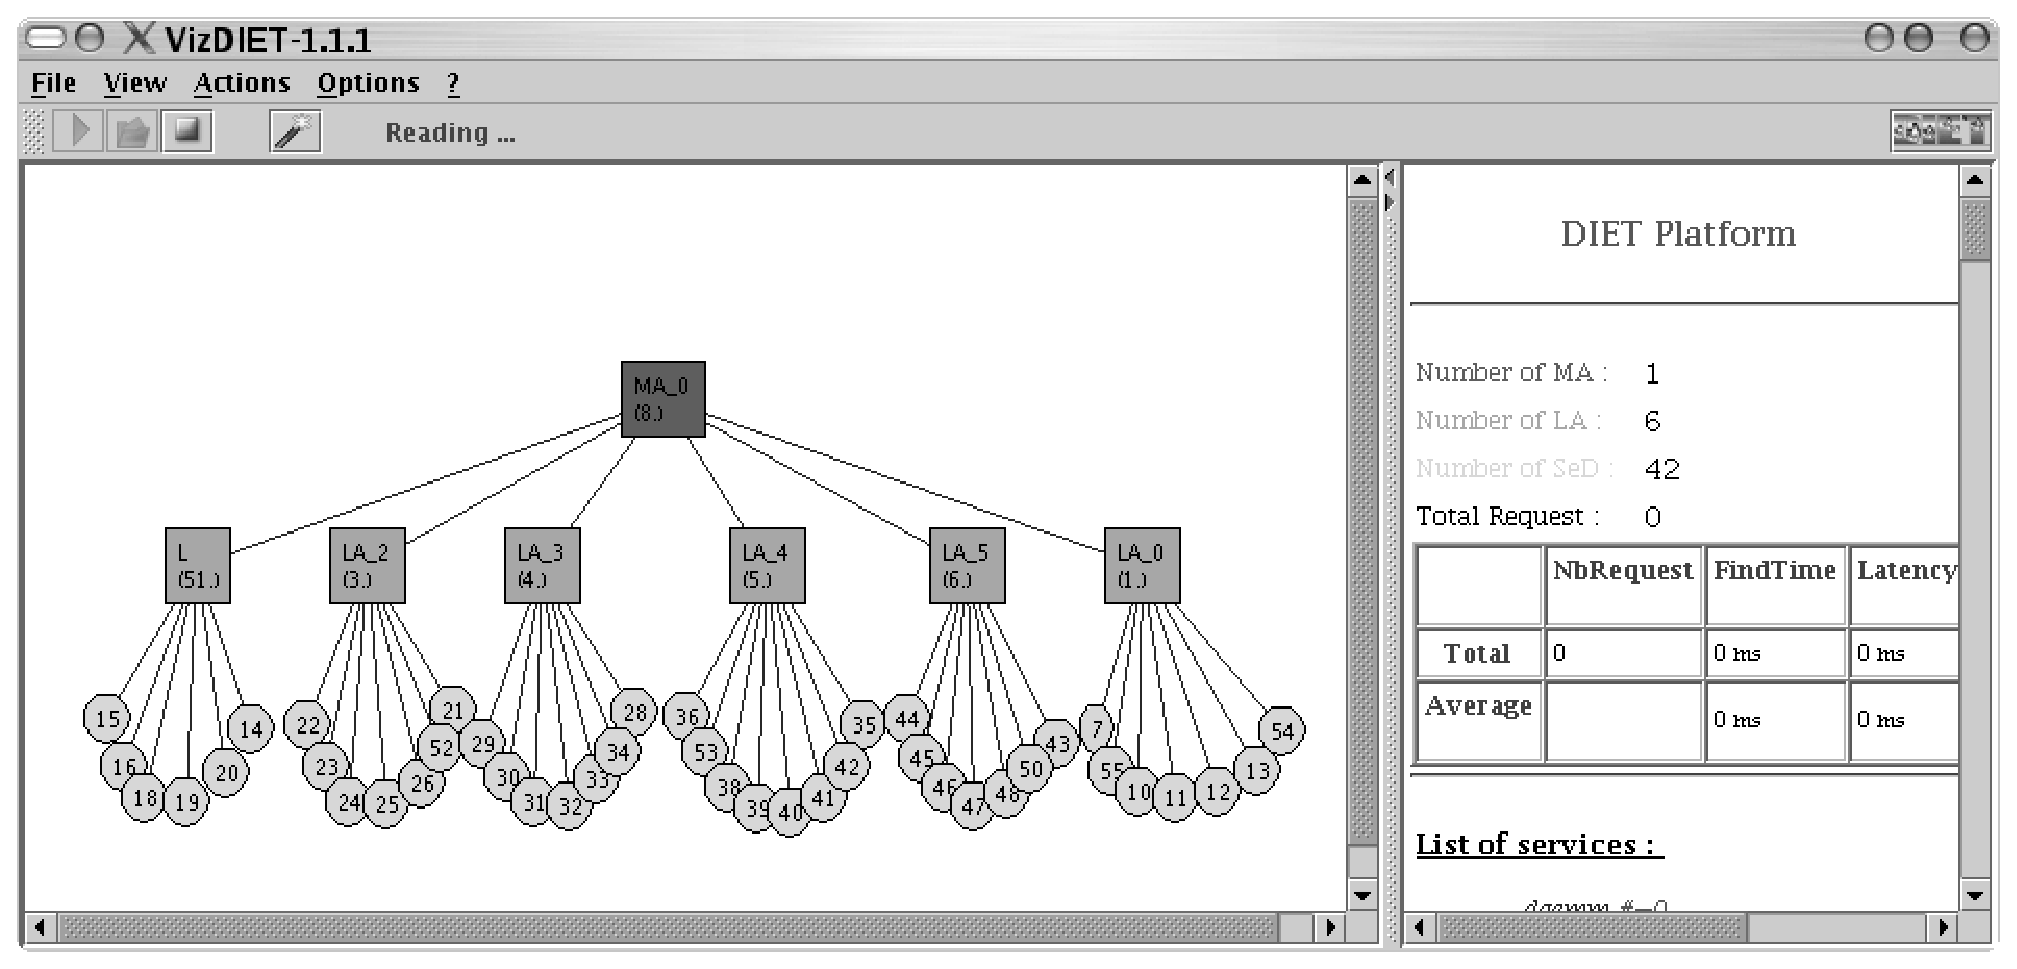
\includegraphics{fig/VizDIET.eps}}
    \caption{snapshot of vizDIET}
    \label{fig:snapshot}
  \end{center}
\end{figure}

As describe in section \ref{sec:solvepb}
 there are two main steps;
one step to find and schedule a service, and one step to solve this service.
So two main activities are represented: schedule and compute informations\\
\begin{description}
  \item [Schedule information]:\\
    When an agent takes a scheduling decision for a task (i.e. finding and deciding which
    SeD can execute a service), it is useful to know how the agent made its decision.
    This information is represented by \textit{FindRequest}.
  \item [Compute information]:\\
    When a SeD is computing a job we need to be aware of its state and know when
    the computation begins and ends. This information is represented by
    \textit{SolveRequest}. In VizDIET, when a SeD is solving a service, this SeD change is color
    and becomes red.\\
\end{description}

  \textit{FindRequest} are only attached to agents and \textit{SolveRequest} are attached to SeDs.
Finally the aggregation of one \textit{FindRequest} and its \textit{SolveRequest} is concatened 
in one request : \textit{DIETRequest}
\textit{DIETResquest} can be see as a job execution in a DIET platform
as seen by an end-user. A \textit{DIETRequest} carries also an other information:
\textbf{latency} which is time between the end of a \textit{FindRequest} and
the begin of a \textit{SolveRequest}.

VizDIET offers the possiblity to vizualise all this request in the point of view of the DIET platform,
in this case you will see the \textit{DIETRequests}, or in the point of view of the Agents or SeDs,
in this case you will see respectivly the \textit{FindRequest} and the \textit{SolveRequest}.
The different kind of requests are represented in different type of graphics such as 
gantt chart, taskflow chart, or bar chart.

\begin{figure}[htb]
  \begin{center}
    \resizebox{.8\linewidth}{!}{\includegraphics{fig/SeD-Gantt-and-load_graph.eps}}
    \caption{bar, taskflow and gantt graph in vizDIET}
    \label{fig:vizStats}
  \end{center}
\end{figure}

VizDIET computes also some other statistic info of the platform such as average time for scheduling, for
solving, or latency. This information can be see for the whole service in the platform or for one sp�cific
service.
VizDIET has got one other interesting feature : this is the possiblity to extract all information collecting
by VizDIET into a file in the way you decide

Finally, VizDIET is quiet useful to understand the behavior of the DIET hierarchy and quite simple to use.
You have to keep in mind that VizDIET based his information uppon log that are forwarded by LogCentral from DIET component.
In consequence all information displayed and compute in VizDIET is only related to the DIET hiearachy (no information from
the client).

VizDIET should implement new functionnality depending of the developement of DIET. For example, the recent interaction between
DIET and Juxmem is also incorporate in VizDIET, to be able to see this interaction.
You can find VizDIET on the web site http://graal.ens-lyon.fr/DIET.
%\section{Statistic}

